% !TeX root = ../main-paper.tex
\begin{figure}[!h]
    \centering
    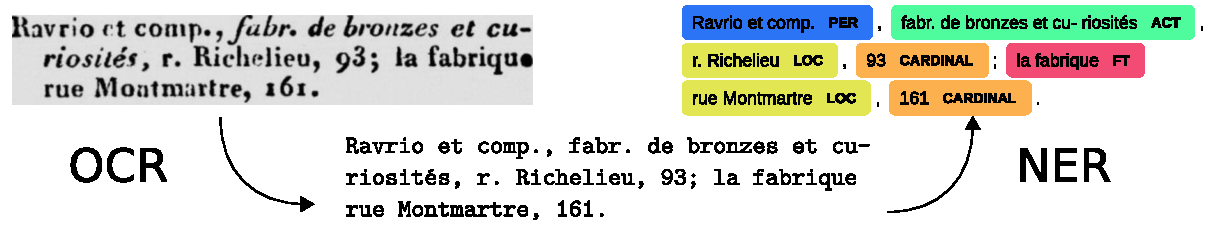
\includegraphics[width=.9\textwidth]{figs/overview-intro.pdf}
    \caption{%
    Overview of the pipeline under study.
    From previously-extracted images of directory entries, 
    we perform OCR and named entity recognition (NER) using different techniques.
    We aim at answering the following questions:
    \emph{How noisy are modern, out-of-the-box OCR systems?}
    \emph{What is the behaviour of NER when OCR is noisy?}
    \emph{Can NER be made more robust to OCR noise?}
    }
    \label{fig.pipeline-overview}
\end{figure}
\clearpage% force float flush!

\section{Introduction}

% General context + scope limitation
OCRed texts are generally not sufficient to build a high level semantic view of a collection of historical documents.
A subsequent stage is often needed to extract the pieces of information most likely to be searched for by users, such as named entities: persons, organisations, dates, places, etc.
Indeed, being able to properly tag text tokens unlocks the ability to relate entities and provide colleagues from other fields with databases ready for exploitation.

Being active research topics, OCR and named entity recognition (NER) are still difficult tasks when applied to historical text documents.
OCR approaches used for modern documents are likely to struggle even on printed historical documents due to multiple causes related to text readability (low resolution scans, inconsistent printing rules, artefacts, show-through), document complexity (intricate and versatile page layout, use of ancient fonts and special glyphs) and the variability inherent to the great diversity of historical sources.
On the other hand, the semantics of entities in NER approaches developed for modern texts may be different from those in ancient texts.

In this article, we focus on a corpus of printed trade directories of Paris from the XIX\textsuperscript{th} century, containing hundreds of pages long lists of people with their activity and address.
They provide fine-grained knowledge to study the social dynamics of the city over time.
As they originate from different publishers, they show a diversity in layout, information organisation and printing quality, which adds to the poor digitising quality to make OCR and NER challenging tasks.

Trade directories have been leveraged in recent work to identify polluted urban soils \cite{bell2020automated} and locate all gas stations in the city of Providence over the last century.
In an ongoing research project, we aim at producing structured spatio-temporal data from the entries of the Paris trade directories to study the dynamics of the fraction of the XIX\textsuperscript{th} century Parisian society reachable through these sources.
%Because they originate from several publishers, their content is organised following different indexing methods (by name, by activity or by address), is printed in various layouts, and uses different fonts.
Therefore, we investigate several state-of-the-art OCR and NER approaches to assess their usability to process the corpus (\cref{fig.pipeline-overview}).

The contributions of this article are as follows:
% Contributions
\begin{enumerate*}[(i)]
    \item We review state-of-the-art OCR and NER systems for historical documents (\cref{sec:related-work}).
    \item We introduce a new dataset suitable for OCR and NER evaluation (\cref{sec:dataset}).
    \item We measure the performance of three modern OCR systems on real data (\cref{sec:ocr-xp}).
    \item We evaluate modern NER approaches: their requirements in terms of training data, and the effects of pre-training (\cref{sec:ner-xp1}).
    \item We show that Transformer-based NER can benefit from pre-training and fine-tuning to improve its performance on noisy OCR (\cref{sec:ner-xp2}).
\end{enumerate*}


